\documentclass[conference]{IEEEtran}
\IEEEoverridecommandlockouts
% The preceding line is only needed to identify funding in the first footnote. If that is unneeded, please comment it out.
\usepackage{cite}
\usepackage[encapsulated]{CJK}
\usepackage{listings}
\usepackage{amsmath,amssymb,amsfonts}
\usepackage{algorithmic}
\usepackage{graphicx}
\usepackage{textcomp}
\usepackage{xcolor}
\usepackage{enumitem}
\usepackage{hyperref}
\def\BibTeX{{\rm B\kern-.05em{\sc i\kern-.025em b}\kern-.08em
    T\kern-.1667em\lower.7ex\hbox{E}\kern-.125emX}}
\begin{document}
\begin{CJK}{UTF8}{bsmi}
\lstset{language=Python} 

\title{Digital Image Final Project Report - Automated Optical Inspection}

\author{\IEEEauthorblockN{107061522 沈煒翔}\IEEEauthorblockN{107061629 蔡喻翔}
\IEEEauthorblockN{107061539 施文弘}
}

\maketitle

\section{Introduction}
Automated Optical Inspection (AOI) is the process to inspect optical defects in industrial production. Traditional inspection method is time-costly and inaccurate. By combining image processing techniques and computer vision techniques, we are able to build to system that automatically inspects optical defects.

In this project, we classify the optical defects into five different categories, void, horizontal defect, vertical defect, edge defect, particle. After classification, we need to mark the defect region, so that maybe the defect can be fixed.

For classification, we build a Convolutional Neural Network (CNN) model. For segmentation, we apply various image processing to mark the defect regions according to the predicted classification result of the CNN.

\section{Optical Defect Classification}

\subsection{Convolutional Neural Network Model}
Convolutional Neural Network (CNN) has shown great results in the field of image classification. The convolutional layers is naturally suitable for image data, since it acts like feature extraction filters. We use CNN to classify optical defects into different categories.

We construct and train a new CNN model (fig. \ref{fig:CNN}). The CNN consists of 3 convolution layers and 2 fully-connected layers. The 3x3 kernel size of the convolutional layers are inspired by VGG-Net\cite{VGG}, which showed that 3x3 convolution kernel is standard in image classification CNNs. Also, we use random search to optimize the hyperparameters, including layers count, node count and learning rate. Drop out layers are added the make the training stage more stable.

\begin{figure}[!htbp]
\centerline{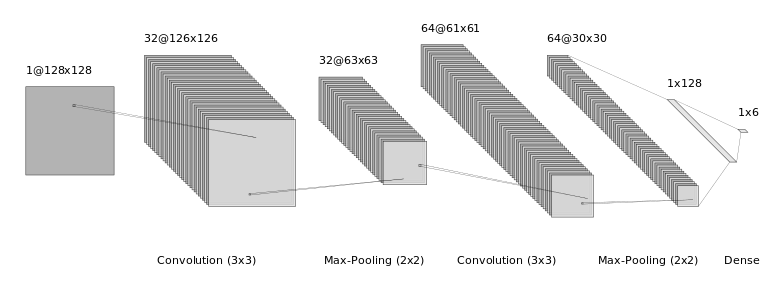
\includegraphics[width=0.5\textwidth]{../figures/nn_architecture.png}}
\caption{Neural Network Architecture. Notice that drop out layers are not drawn in this figure.}
\label{fig:CNN}
\end{figure}

\subsection{Image Augmentation}
In the optical defect dataset, the categories are imbalanced. The CNN would refuse to predict the smaller categories. Therefore, we try to resample the smaller categories by naively oversampling them, so that the CNN have more training samples in those smaller categories. However, naively oversampling cause the categories to converge in different speed; one category may begin to over-fit while the others may still be under-fitting. Therefore, we conclude that naively oversampling would not work, and turn to image augmentation.

Image Augmentation were used on both training and validation datasets. The augmentation includes vertical and horizontal flip, and padding. After the augmentation, the dataset is approximately 15 times larger than the original dataset. By enlarging the dataset, we can prevent overfitting, and make the training stage more stable.

\begin{figure}[!htbp]
\centerline{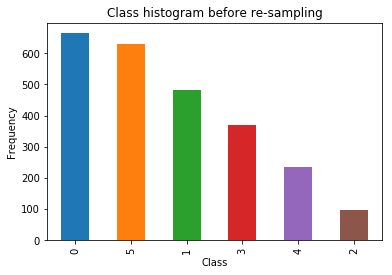
\includegraphics[width=0.4\textwidth]{../figures/training_data_before_augmentation.png}}
\centerline{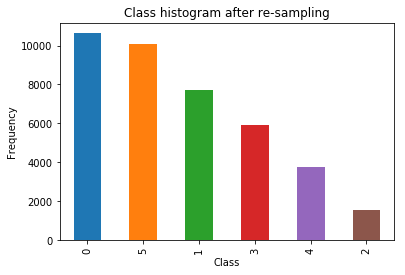
\includegraphics[width=0.4\textwidth]{../figures/training_data_after_augmentation.png}}
\caption{Comparison of doing and not doing image augmentation. Notice the change of data size.}
\end{figure}

\section{Optical Defect Segmentation}

Different image processing procedures are applied to different defect categories. We assume the prediction of CNN is correct, and apply the following image processing methods.

\subsection{Void Defect}
First, The noise is removed by using Gaussian filter (fig. \ref{fig:Void}b) and median filter (fig. \ref{fig:Void}c). Gaussian filter is used to reduce image noise. Median filter is used remove extreme value. After using the filters, the image is smoothed.

We want to find the threshold between normal region and defect region. To determine the threshold, we observe the histogram distribution of pixel intensity (fig. \ref{fig:Histogram}). There are two obvious peaks that contribute to normal region and void region.

We assume the local minimal point between two peaks is the threshold. To prevent finding points at the very start or very end of the histogram, the 20\% beginning and end value were deleted. By doing so, we can find the adaptive threshold to distinguish void region and normal region.

\begin{figure}[!htbp]
\centerline{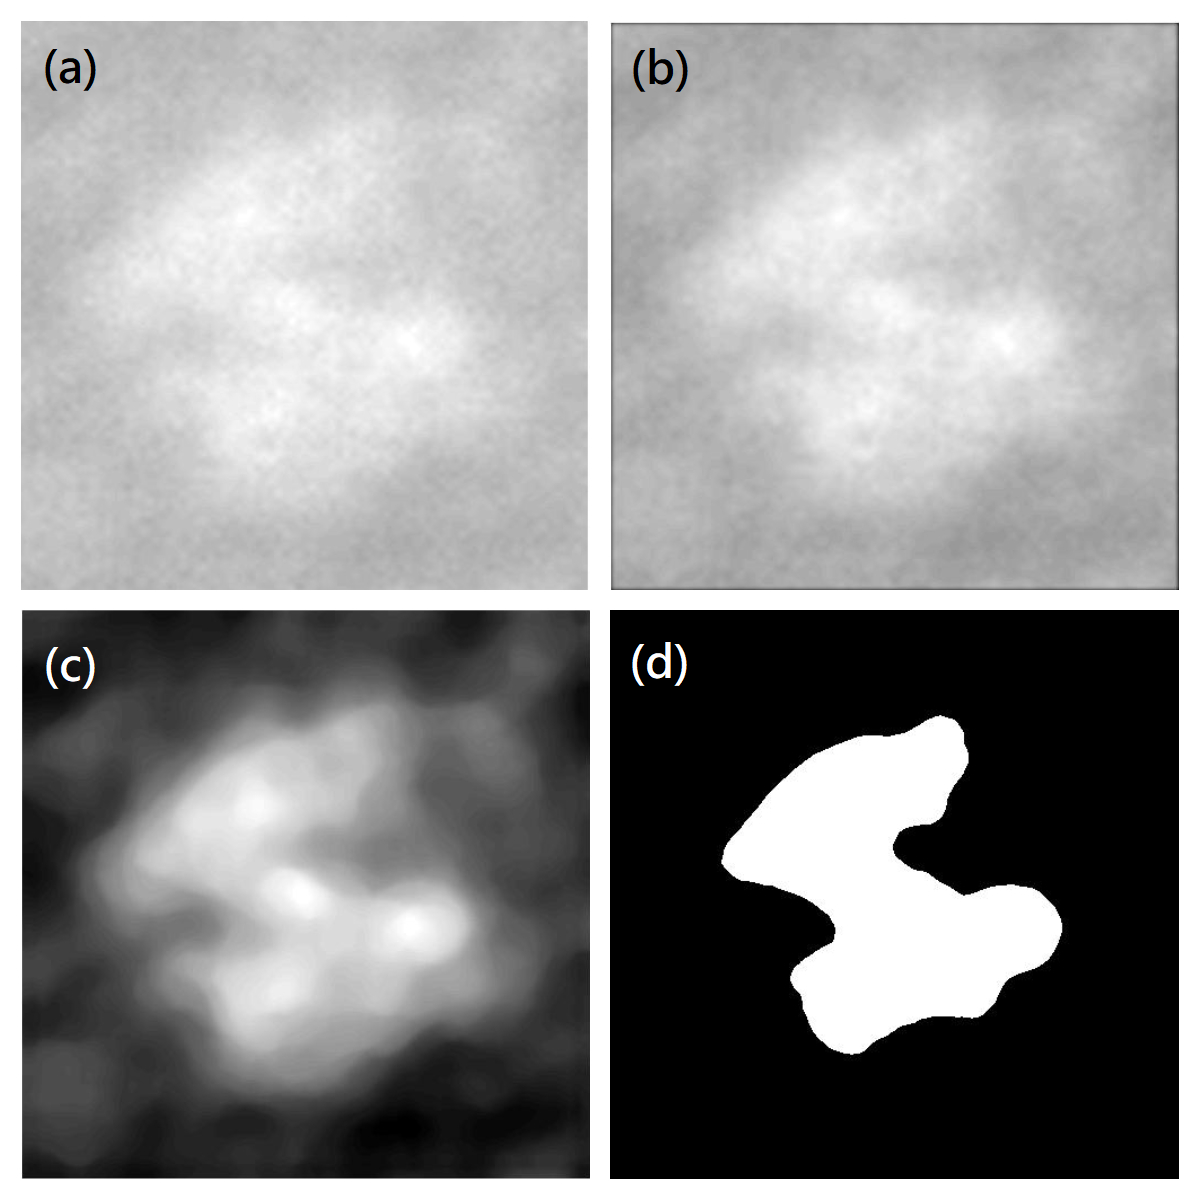
\includegraphics[width=0.4\textwidth]{../figures/Void.png}}
\caption{Void Defect Segmentation. (a)Original Image, (b)After Gaussian filter, (c)After Median filter, (d)After adaptive thresholding.}
\label{fig:Void}
\end{figure}

\begin{figure}[!htbp]
\centerline{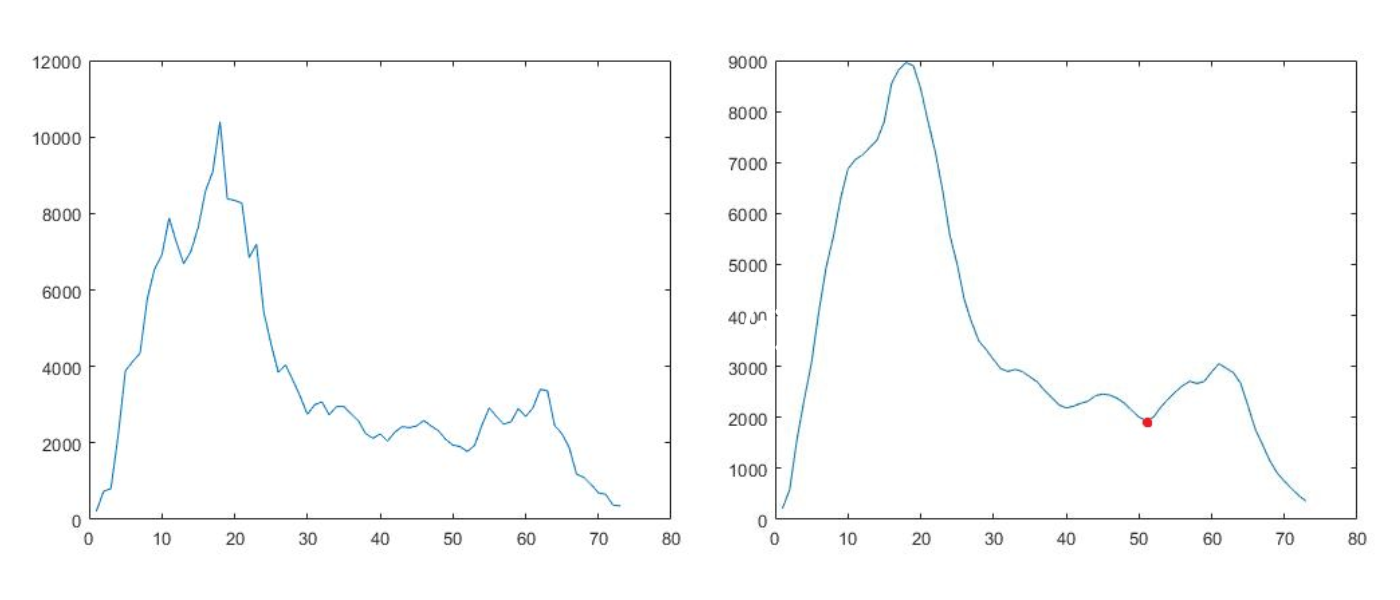
\includegraphics[width=0.4\textwidth]{../figures/histogram.png}}
\caption{Histogram distribution of pixel intensity. The red point in the right point is the adaptive threshold.}
\label{fig:Histogram}
\end{figure}

\subsection{Horizontal Defect}
In horizontal defect, there is an obvious horizontal line/lines in the image. If we average all pixel intensity in each row, we can see an drop-off in the intensity in each row (fig. \ref{fig:Horizontal}b).

We use derivative method to find the drop-off intensity area. We use 5x5 median filter followed by 5x5 averaging filter. Before differentiating the image, it should be averaged every 100 columns. Then we can differentiate the image by convolution with a gradient operator [-1;1] (fig. \ref{fig:Horizontal}c). At last, we smooth the image with 1x9 averaging mask to get a difference image.

For both ramp edge and roof edge, its position should be near the peak value of the first derivative. So we set a threshold with magnitude half of the peak value. If the peak value is positive, all pixels higher than threshold are set to 1, others are set to zero. If the peak value is negative, all pixels lower than threshold are set to 1, others are set to zero (fig. \ref{fig:Horizontal}d). Finally, we resize the image back to 512x512.

\begin{figure}[!htbp]
\centerline{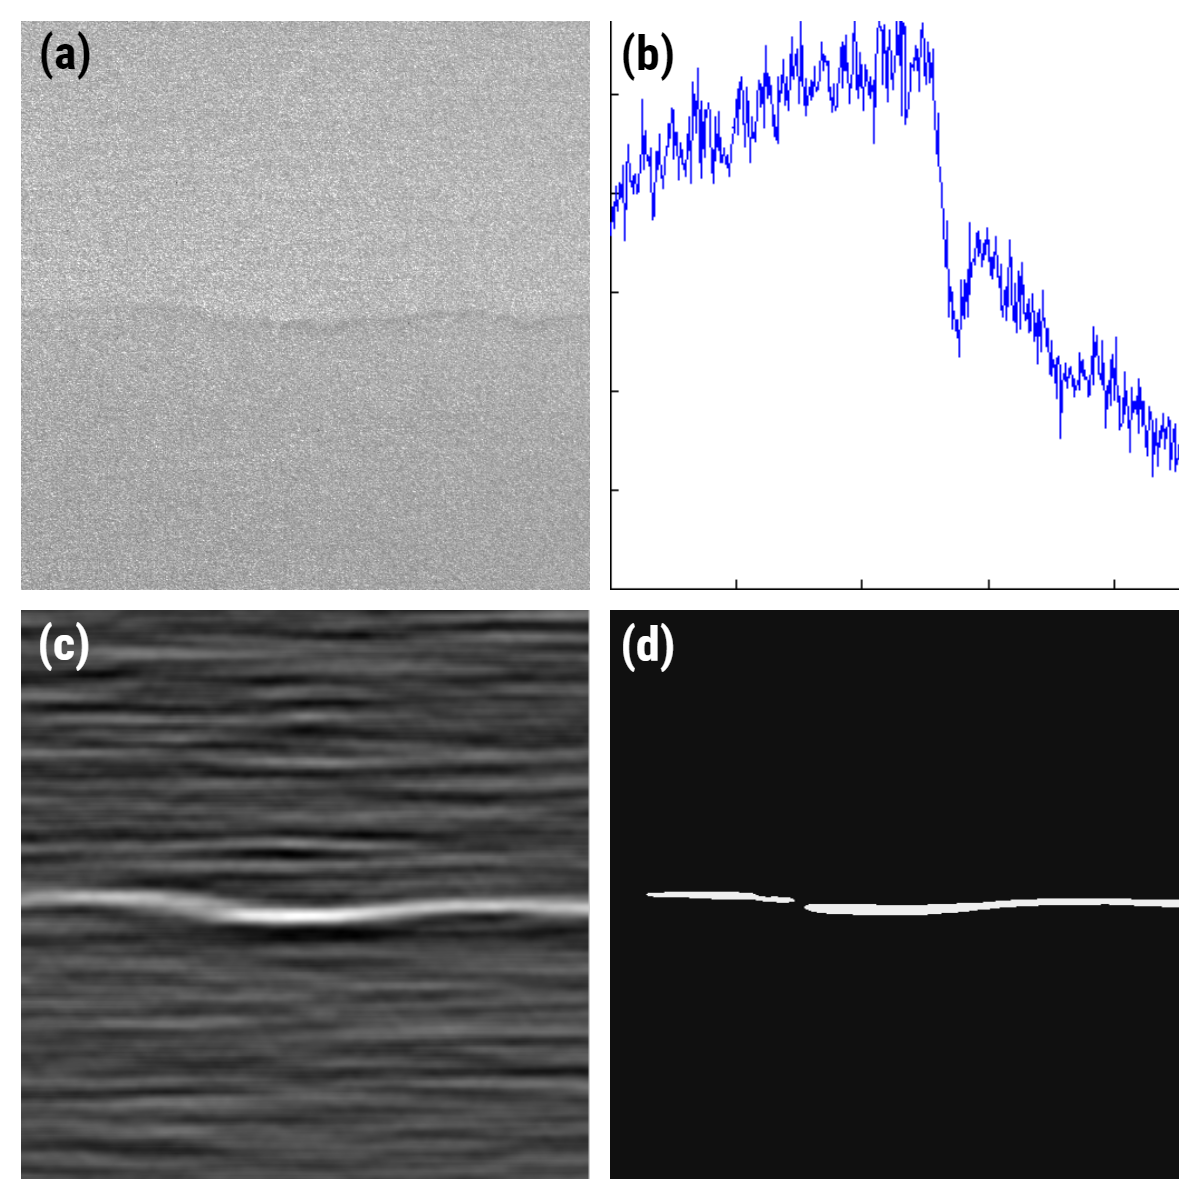
\includegraphics[width=0.4\textwidth]{../figures/Horizon.png}}
\caption{Horizontal Defect Segmentation. (a)Original Image, (b)Average intensity of each row, (c)Difference image after gradient operator, (d)Image after thresholding.}
\label{fig:Horizontal}
\end{figure}

\subsection{Vertical Defect}
We rotate the image 90 degree so that it becomes a horizontal defect image, and pass it into the same algorithm used in horizontal defect. At last, transpose it again and we can get the final result.

Note that because vertical edges are more visible than horizontal edges, we average by every 50 columns instead of 100 columns, and the threshold is set to 0.3 instead of 0.5 in horizontal defects (fig. \ref{fig:Vertical}).

\begin{figure}[!htbp]
\centerline{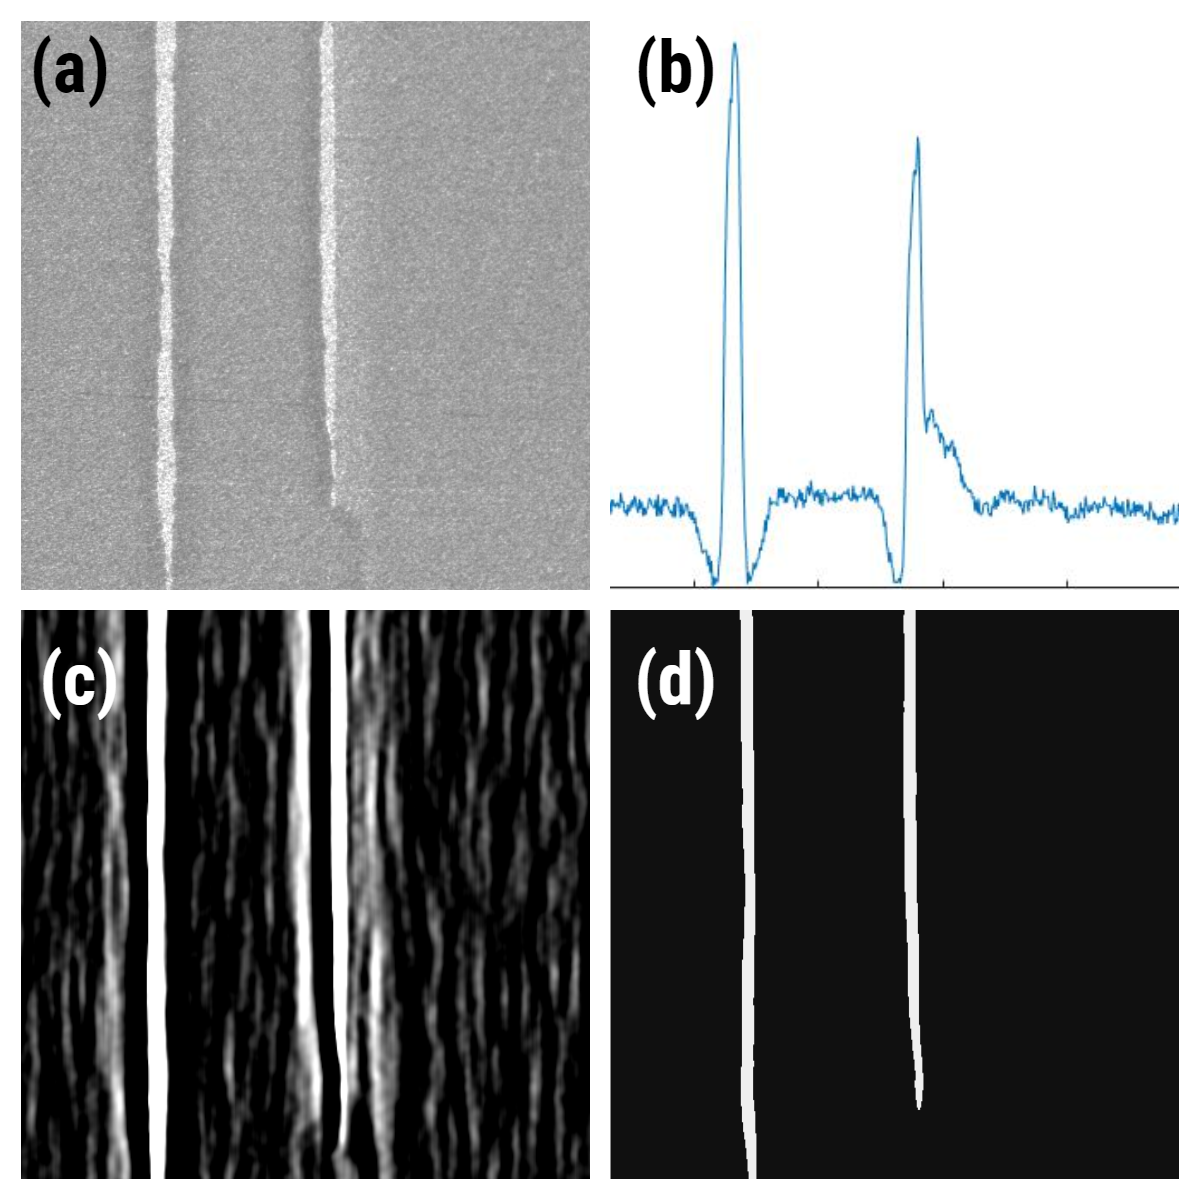
\includegraphics[width=0.4\textwidth]{../figures/Vertical.png}}
\caption{Horizontal Defect Segmentation. (a)Original Image, (b)Average intensity of each row, (c)Difference image after gradient operator, (d)Image after thresholding.}
\label{fig:Vertical}
\end{figure}

\subsection{Edge Defect}
We can see obvious feature on the images, so we find the edge boundary. To remove the noise and extreme value, we use median filter (fig. \ref{fig:Edge}b). we use Canny edge detector \cite{Canny} and larger value of standard deviation of the Gaussian filter (fig. \ref{fig:Edge}c). Then we dilation the boundary with a 3x3 matrix of ones to make the boundary more visually visible (fig. \ref{fig:Edge}d). 

\begin{figure}[!htbp]
\centerline{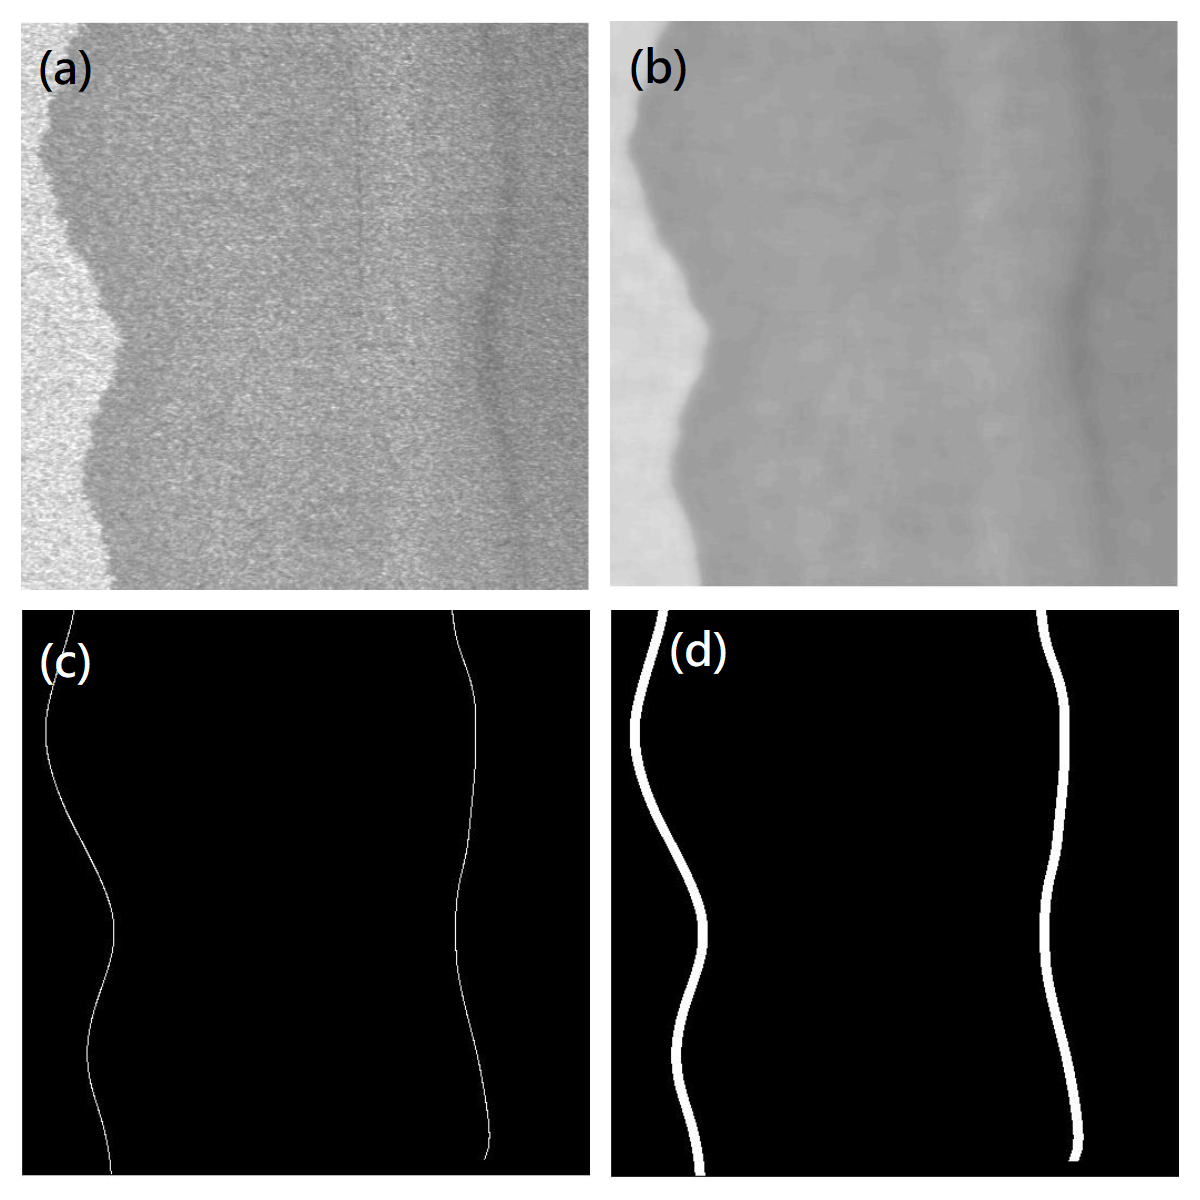
\includegraphics[width=0.4\textwidth]{../figures/Edge.png}}
\caption{Edge Defect Segmentation. (a)Original Image, (b)Image after median filter, (c)Canny edge detection using large deviation of Gaussian filter, (d)Dilation to make the boundary more visually visible.}
\label{fig:Edge}
\end{figure}

\subsection{Particle Defect}
We can see that there is a dark region in the middle of image, and many speckles around the image. In particle defect category, we would mark both defects.

First, we remove the noise by using median filter. (fig. \ref{fig:Particle}b) To mark the speckles in the image, we define the mean of the image as the threshold (fig. \ref{fig:Particle}c).

For the dark region in the middle of the image, we find the local minimal point between two peaks in histogram distribution of pixel intensity. The method is similar as those used in void defect. It can clearly mark dark region in the middle (fig. \ref{fig:Particle}d).

\begin{figure}[!htbp]
\centerline{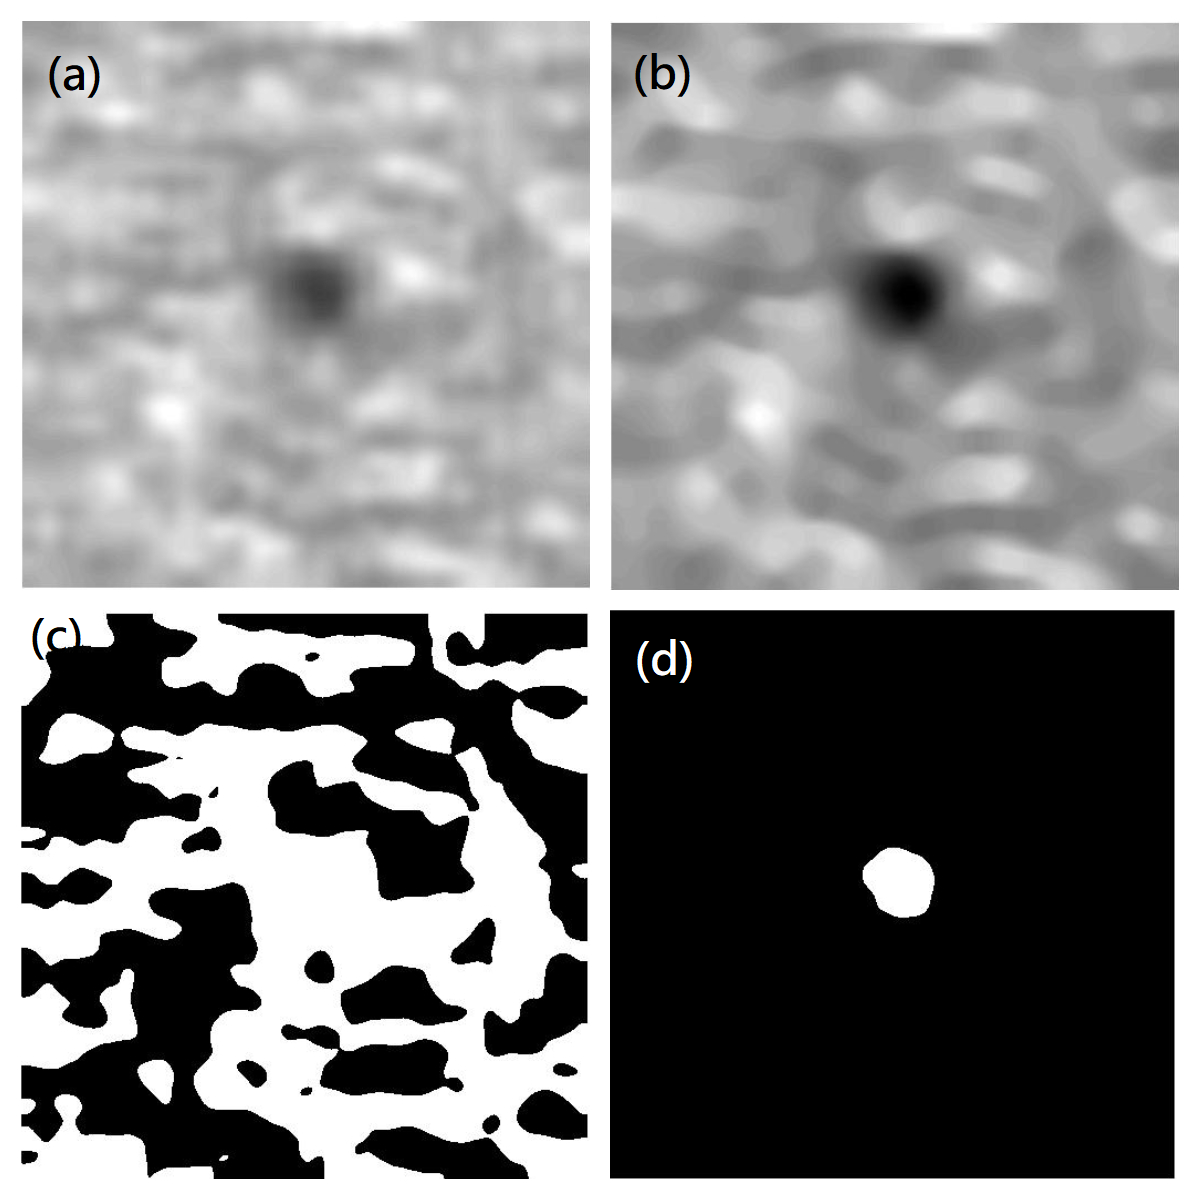
\includegraphics[width=0.4\textwidth]{../figures/Particle.png}}
\caption{Edge Defect Segmentation. (a)Original Image, (b)Image after median filter, (c)Speckle defect by adaptive thresholding, (d)Dark region defect by adpative thresholding.}
\label{fig:Particle}
\end{figure}

\section{Results and Discussion}
\subsection{CNN Result}
The CNN model is trained 25 epochs by Adam optimizer using learning rate of 0.01. Detail training settings can be viewed in the provided code.

We separate the training dataset into training and validation set in the ratio of 0.8 and 0.2. 5-fold cross validation is used for estimating the performance of the model. The proposed CNN model achieve 98.21\% during cross validation and achieve 98.99\% accuracy in the private leader board of AIdea website (fig. \ref{fig:Epoch}).

\begin{figure}[!htbp]
\centerline{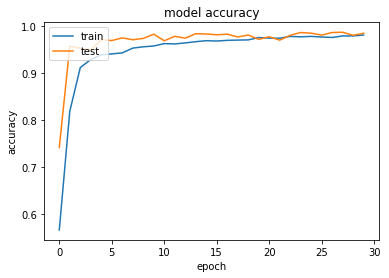
\includegraphics[width=0.4\textwidth]{../figures/accuracy.png}}
\centerline{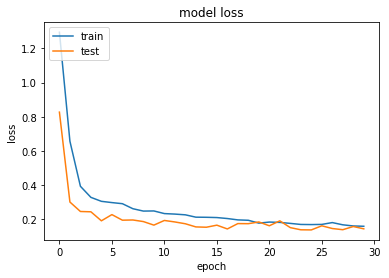
\includegraphics[width=0.4\textwidth]{../figures/loss.png}}
\centerline{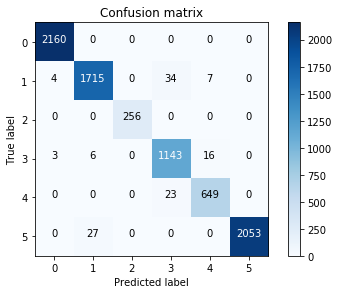
\includegraphics[width=0.4\textwidth]{../figures/confusion_matrix.png}}
\caption{Accuracy and loss with each epoch. Note that the orange line is actually validation accuracy and loss. Confusion matrix is plotted using validation dataset.}
\label{fig:Epoch}
\end{figure}

\subsection{Segmentation Result}
Segmentation of void defect sometimes cannot mark defect region. We conclude several circumstances that the algorithm could fail. One, some images classified in void looks normal. Second, the adaptive threshold sometimes fail to find an optimal point to distinguish to normal and defect region. In some case (fig. \ref{fig:Void2}), the void defect region is not defined very well.

\begin{figure}[!htbp]
\centerline{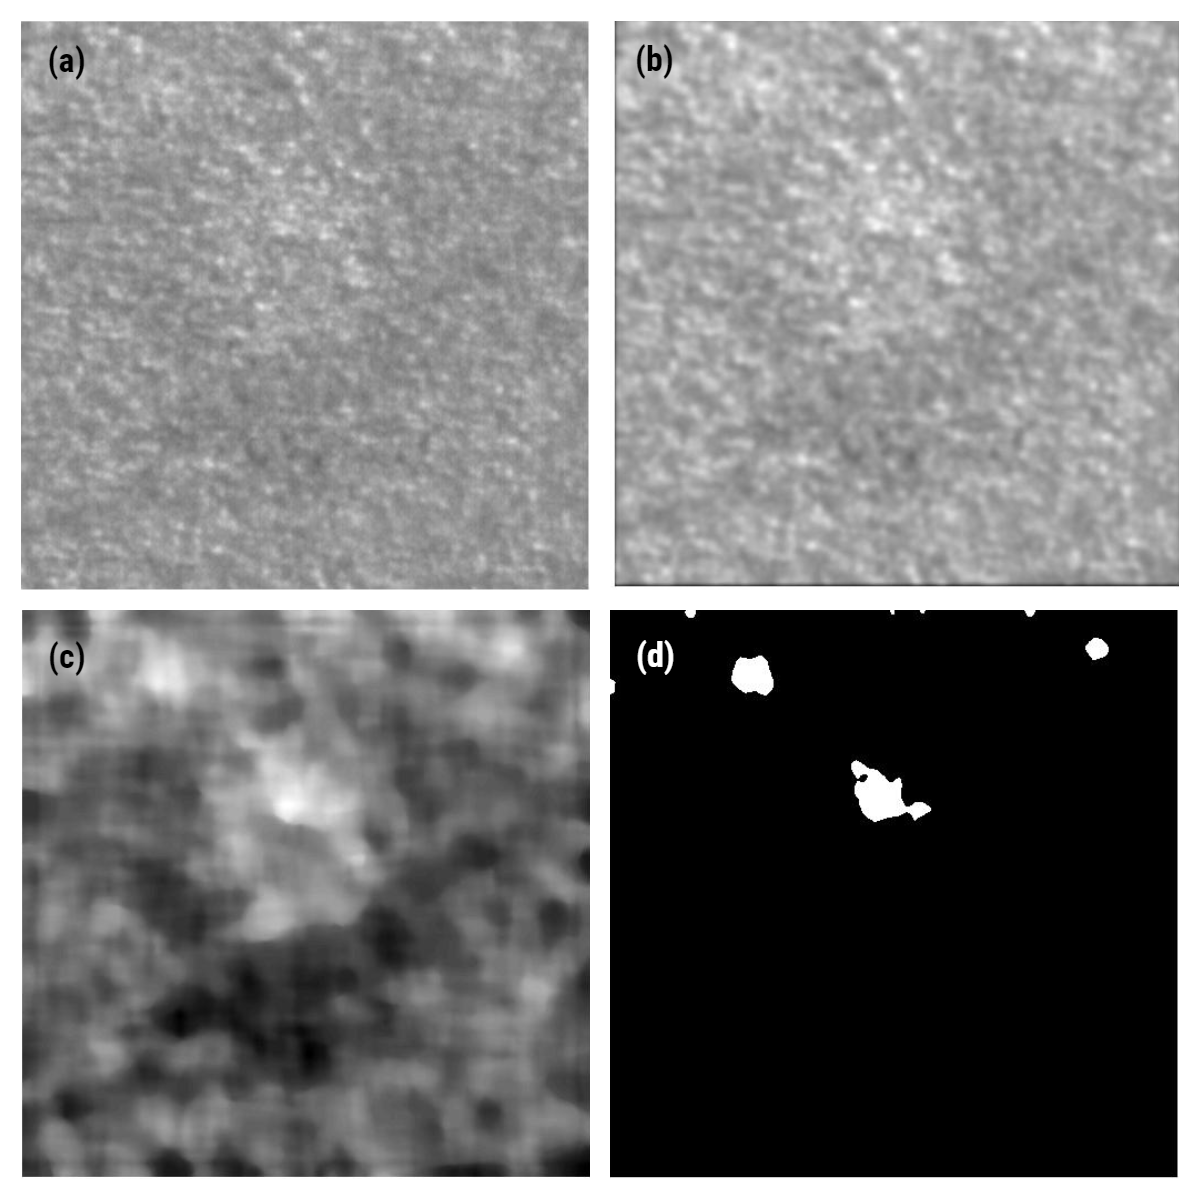
\includegraphics[width=0.3\textwidth]{../figures/Void2.png}}
\caption{Fail segmentation of void category due to unclear definition of defect region.}
\label{fig:Void2}
\end{figure}

For edge defect, There are some images' edges are visually unclear (fig. \ref{fig:Edge2}), which have many wrong edges in it. However, changing the threshold can remove wrong edges. That is because the threshold is same to all images, but it should be adjust between different images. Maybe we can decide threshold by the images' standard deviation or other statistical method.

\begin{figure}[!htbp]
\centerline{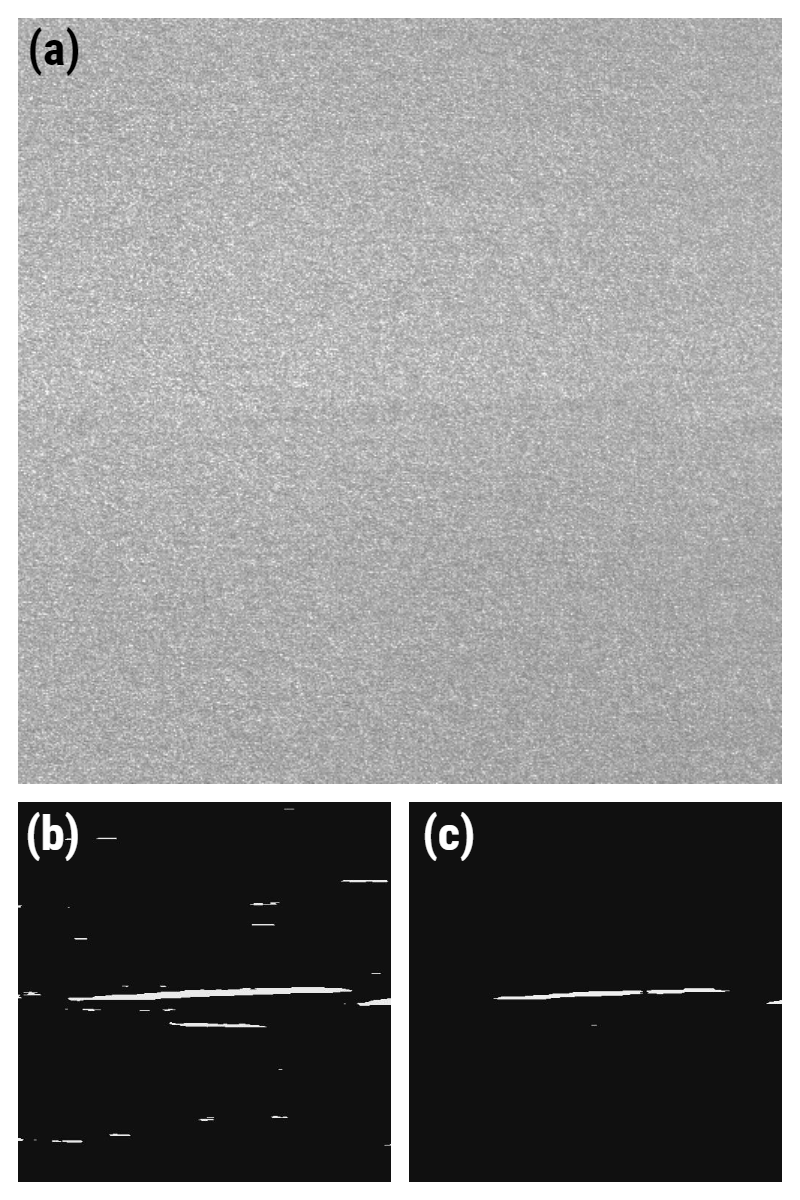
\includegraphics[width=0.25\textwidth]{../figures/Wrong.png}}
\caption{Fail segmentation of edge category due to unclear definition of defect region and fixed threshold.}
\label{fig:Edge2}
\end{figure}

\section{Conclusion}
In this project, we classify the optical defect images into six different categories. We build and train a new CNN for image classification, and achieve 98.99\% accuracy on the private leader board of AIdea, which is the 3rd team in class.

Image segmentation is used to mark the defect region. The segmentation rely on the prediction of CNN, since different algorithms are used in different defect categories. For most images, we are able to mark the defect region clearly.

\newpage
\begin{thebibliography}{00}

\bibitem{VGG} 
Karen Simonyan and Andrew Zisserman.
\textit{Very Deep Convolutional Networks for Large-Scale Image Recognition}. 
CoRR, 1993.
 
\bibitem{Canny} 
John Canny.
\textit{A Computational Approach to Edge Detection}.
IEEE Transactions on Pattern Analysis and Machine Intelligence, Nov. 1986.

\end{thebibliography}

%\subsection{Entropy of Image}
%Entropy is one the metrics to measure average information  per pixel in an image. Entropy (or uncertainty) is higher when the image is more messy. For example, a pure white image has 0 entropy, while a noise image has very high entropy.
%
%Let \(P(a_i)\) be the probability of the pixel with intensity = i. Entropy \(H(z)\) can be calculated by:
%
%\[ H(z) = -\sum\limits_{i=1}^n P(a_i)log_2P(a_i) \]
%
%Most of the time, images with higher entropy is more difficult to achieve higher compression ratio.

%\subsection{Huffman Coding}
%When performing Huffman encoding, we need to first observe (or guess) the probability distribution of pixel intensity. From the distribution, we can build a Huffman tree, which assign block codes to each sequence.
%
%When using Huffman coding, the dictionary (or Huffman tree) would need to be send, so that the receiver can decode the message using the dictionary.
%
%We might not always have the exact probability distribution when encoding messages. If wrong approximation of probability distribution model were used in Huffman encoding, it may lead to compression result that are larger than the original image. Therefore, adaptive Huffman coding is used to counter the issue.
%
%\subsection{Arithmetic Coding}
%Unlike Huffman coding, Arithmetic coding is a non-block code, which the entire sequence of source symbols is assigned a single arithmetic code.
%
%However, in practise, the floating point system has its precision limit. Therefore, the length of each arithmetic code is limited by the precision of the floating number (single precision floating number or double precision floating number). In this homework, I chose to use double precision floating number to perform arithmetic coding.
%
%Arithmetic coding also needs to estimate the probability distribution model first. So it faces the same issue as Huffman coding. Wrong approximation of the probability model may lead to compression result worse than original image.
%
%\subsection{LZW Coding}
%LZW coding is a compression method that reduces	spatial redundancy of the messages. The encode/decoder builds the dictionary dynamically as the text is being transferred. This gives LZW a high compression rate, but takes many time to encode or decode.
%
%In practise, we limit the length of dictionary to certain bits, so that the dictionary would not become too long that the compression starts to drop. 
%
%By the rule of thumb, 10 to 12 bits of LZW dictionary is used in most English articles. In this homework, I chose to use 11 bit LZW dictionary.
%
%\subsection{Image Permutation}
%In this homework, we were given a image that are randomly shifted in each row (or column).
%
%We assume that natural images are continuous, so thus two rows should have high correlation coefficient. We can know that whether the two neighbour rows are correctly shifted.
%
%Since the first row of the image is not shift, we can estimate the next row by circular shifting the next row, and calculate the correlation coefficient between two rows.
%
%\section{Results and Discussion}
%
%%\begin{figure}[!htbp]
%%\centerline{\includegraphics[width=0.3\textwidth]{image1.png}}
%%\caption{Test image 1}
%%\end{figure}
%%
%%\begin{figure}[!htbp]
%%\centerline{\includegraphics[width=0.3\textwidth]{image2.png}}
%%\caption{Test image 2}
%%\end{figure}
%
%\subsection{Entropy}
%\begin{table}[!htbp]
%\begin{tabular}{|c|c|c|}
%\hline
%        & Entropy & \multicolumn{1}{r|}{Horizontal Difference Image Entropy} \\ \hline
%Image 1 & 7.57148 & 4.12952                                                  \\ \hline
%Image 2 & 7.40788 & 4.10455                                                  \\ \hline
%\end{tabular}
%\end{table}
%
%We can see that image 2 has a lower entropy. Therefore, it has the potential to achieve higher compression rate.
%
%\subsection{Huffman Coding}
%\begin{table}[!htbp]
%\begin{tabular}{|c|c|c|c|}
%\hline
%Huffman Encoding & Bit per Pixel & Compression Ratio & Redundancy \\ \hline
%Image 1          & 7.595         & 1.053             & 0.050           \\ \hline
%Image 2          & 7.429         & 1.076             & 0.071           \\ \hline
%\end{tabular}
%\end{table}
%
%We can see that image 2 has a higher compression rate in Huffman encoding. This is reasonable, since image 2 has a lower entropy.
%
%\subsection{Arithmetic Coding}
%\begin{table}[!htbp]
%\begin{tabular}{|c|c|c|c|}
%\hline
%Arithmetic Encoding & Bit per Pixel & Compression Ratio & Redundancy \\ \hline
%Image 1          & 7.624         & 1.049             & 0.046           \\ \hline
%Image 2          & 7.489         & 1.068             & 0.063           \\ \hline
%\end{tabular}
%\end{table}
%
%Comparing to Huffman coding, the compression ratio is slightly lower.
%
%\subsection{LZW Coding}
%\begin{table}[!htbp]
%\begin{tabular}{|c|c|c|c|}
%\hline
%LZW Encoding & Bit per Pixel & Compression Ratio & Redundancy \\ \hline
%Image 1      & 6.911         & 1.157             & 0.136           \\ \hline
%Image 2      & 4.61          & 1.733             & 0.423           \\ \hline
%\end{tabular}
%\end{table}
%
%We can see that LZW coding beats Huffman coding and Arithmetic coding a lot. Since LZW reduces the spatial information by dynamically building dictionary. However, LZW coding takes huge amount of time which is an obvious trade off.
%
%In this homework, I chose to use a maximum of 11-bit LZW dictionary.

%\subsection{Image Permutation}
%\begin{figure}[!htbp]
%\centerline{\includegraphics[width=0.3\textwidth]{image3.png}}
%\caption{Test image 3}
%
%\centerline{\includegraphics[width=0.3\textwidth]{image3_recovered.png}}
%\caption{Recovered test image 3}
%
%\centerline{\includegraphics[width=0.3\textwidth]{image4.png}}
%\caption{Test image 4}
%
%\centerline{\includegraphics[width=0.3\textwidth]{image4_recovered.png}}
%\caption{Recovered test image 4}
%\end{figure}

%The recovered images are pretty good. There may be some little flaws that we cannot see. It would be a good experiment to compare the recovered image with the ground truth image, but we were not given the ground truth image. Anyway, the recovered images are acceptable.

%\subsection{Image Restoration using Notch Filter}
%We can observe that in the original image, there are periodic noise interference, which is the diagonal grids in the image. 
%
%Since the noise is very periodic and contains only one frequency, it can be seen clearly  as a dot (two dots in this case) in the frequency spectrum (Fig. 1).
%
%We can design a Notch filter that eliminates the two dots in the frequency spectrum. In this homework, I designed a Gaussian Notch filter to eliminate the noise (Fig. 2, 3).
%
%\begin{figure}
%\centerline{\includegraphics[width=0.35\textwidth]{Notch_1.png}}
%\caption{Frequency Spectrum before Notch filtering}
%
%\centerline{\includegraphics[width=0.35\textwidth]{Notch_2.png}}
%\caption{Frequency Spectrum of the Gaussian Notch filter}
%
%\centerline{\includegraphics[width=0.35\textwidth]{Notch_3.png}}
%\caption{Frequency Spectrum after Notch filtering}
%\end{figure}
%
%\subsection{Image Restoration using Band-reject Filter}
%The design method is similar to Notch filter. We first observe the frequency spectrum and see that there is obvious noise points in the spectrum (Fig. 4).
%
%Since the six noise points are in the region of the same frequency band, a band-reject filter can easily filter out all six of the noise. In this homework, I designed a ideal band-reject filter to eliminate the noise (Fig. 5, 6).
%
%\begin{figure}
%\centerline{\includegraphics[width=0.35\textwidth]{Band_Reject_1.png}}
%\caption{Frequency Spectrum before Band-reject filtering}
%
%\centerline{\includegraphics[width=0.35\textwidth]{Band_Reject_2.png}}
%\caption{Frequency Spectrum of the Ideal Band-reject filter}
%
%\centerline{\includegraphics[width=0.35\textwidth]{Band_Reject_3.png}}
%\caption{Frequency Spectrum after Band-reject filtering}
%\end{figure}
%
%\subsection{Homomorphic Filtering}
%We assume that an image is the multiplication of its illumination and reflectance.
%\[ Image(x,y) = i(x,y) \cdot r(x,y) \]
%
%We can improve the appearance of an image by gray-level range compression and contrast enhancement.
%
%Illumination are mostly slow spatial variation (low freq. component) and reflectance are mostly high freq. component. However, \(i(x,y)\) and \(r(x,y)\) are not separable, so it is hard to do calculations after Fourier Transform. Instead, we take Fourier Transform on the log image, since log operation helps us turns the product to sum.
%\[ ln(Image(x,y)) = ln(i(x,y)) + ln(r(x,y)) \]
%\[ F.T(ln(Image(x,y))) = F.T(ln(i(x,y))) + F.T(ln(r(x,y))) \]
%
%That is, \[ Image(u,v) = I(u,v) + R(u,v) \]
%
%Therefore, we design filters in the frequency domain to amplify high freq. component and attenuate low freq. component. In this homework, we design an ideal high-pass filter, Butterworth high-pass filter, and a Gaussian high-pass filter (Fig. 7, 8, 9).
%
%\begin{figure}
%\centerline{\includegraphics[width=0.35\textwidth]{Homomorphic_1.png}}
%\caption{Ideal high-pass filter for homomorphic filtering}
%
%\centerline{\includegraphics[width=0.35\textwidth]{Homomorphic_2.png}}
%\caption{Butterworth high-pass filter for homomorphic filtering}
%
%\centerline{\includegraphics[width=0.35\textwidth]{Homomorphic_3.png}}
%\caption{Gaussian high-pass filter for homomorphic filtering}
%\end{figure}
%
%\section{Results}
%
%High resolution output images can be found in the "./out" folder. 
%
%\begin{figure}
%\centerline{\includegraphics[width=0.35\textwidth]{Wiener_1.png}}
%\caption{Output fish image of Wiener filter.}
%
%\centerline{\includegraphics[width=0.35\textwidth]{Wiener_2.png}}
%\caption{Output letter image of Wiener filter.}
%
%\centerline{\includegraphics[width=0.35\textwidth]{Notch_4.png}}
%\caption{Output denoised image of Notch filter.}
%
%\centerline{\includegraphics[width=0.35\textwidth]{Band_Reject_4.png}}
%\caption{Output denoised image of band-reject filter.}
%\end{figure}
%
%\begin{figure}
%\centerline{\includegraphics[width=0.35\textwidth]{Homomorphic_4.png}}
%\caption{Homomorphic filtering of Ideal high-pass filter}
%
%\centerline{\includegraphics[width=0.35\textwidth]{Homomorphic_5.png}}
%\caption{Homomorphic filtering of Butterworth high-pass filter}
%
%\centerline{\includegraphics[width=0.35\textwidth]{Homomorphic_6.png}}
%\caption{Homomorphic filtering of Gaussian high-pass filter}
%
%\end{figure}
%
%\section{Discussion}
%
%\subsection{Degradation System Estimation in Wiener Filtering}
%In Wiener filtering, I cannot obtain very impressive result, due to the inaccuracy estimation of the degradation system.
%
%In the letter image, there is a impulse point at the top-left of the image. The point is blurred by the degradation system. Therefore, we can use the region as the PSF of the system and calculate its inverse system. However, it is not an ideal impulse point, so there is still ripple defects in the edges of the images.
%
%In the fish image, it hard to observe what kind of degradation function it is. By try-and-error, I think it is most likely to be Gaussian-blur degradation system. Therefore, a inverse system was used for Wiener filtering, but it also did not obtain the ideal result, (which we do not know what the ideal result looks like).
%
%\subsection{Notch Filters and Band-reject Filters}
%In both Notch filtering and band-reject filtering, we want to eliminate particular noise interference in the frequency domain. Notch filters are suitable for removing point-frequency noise, and band-reject filters are suitable for removing an area of noise. In this homework, six Notch filters can be cascaded to reach the same effect of the band-reject filter.
%
%\subsection{Ideal and Non-ideal Filters}
%In this homework, we designed Notch filter and band-reject filters by Gaussian kernel and ideal kernel. Both work very well.
%
%An ideal filter in frequency domain would be sinc function in the time domain. Sinc function and those weird ripples (sidelobes) in the pass-band; therefore it creates little defects around the edges. The ripple defects is hard to observe thus ignorable in this band-stop case.
%
%\subsection{Butterworth and Gaussian Kernel}
%Butterworth filter can control its drop-off leap by increasing or decreasing the order of the filter. While in Gaussian Kernel, it is often a smooth drop-off leap. In my opinion, Butterworth filter yields the most optimal result in homomorphic filtering.
%
%Ideal filter would create ripple edges due to its sinc function in time domain. Gaussian filter has a smooth transition in edges but less contrast enhancement because it discriminate the high freq. component and low freq. component less.

%\begin{thebibliography}{00}
%\bibitem{b1} Bitmap file format, "https://en.wikipedia.org/wiki/BMP\_file\_format"
%\bibitem{b2} Laplacian of Gaussian, "https://homepages.inf.ed.ac.uk/rbf/HIPR2/log.htm"
%\bibitem{b3} Frequency response of moving average filter, "https://ptolemy.berkeley.edu/eecs20/week12/freqResponseRA.html"
%\bibitem{b4} Non-local mean filter for image denoising, "https://www.iro.umontreal.ca/~mignotte/IFT6150/Articles/Buades-NonLocal.pdf"
%\end{thebibliography}"

\end{CJK}
\end{document}
